\documentclass[a4paper, 12pt]{article}

\usepackage[utf8]{inputenc}
\usepackage[T1]{fontenc}
\usepackage{lmodern}

\title{A \LaTeX{} document}
\author{Jonas C. J.}

\usepackage{graphicx}
\usepackage{float}
\begin{document}
Some text before the figure.
\begin{figure}
\begin{center}
	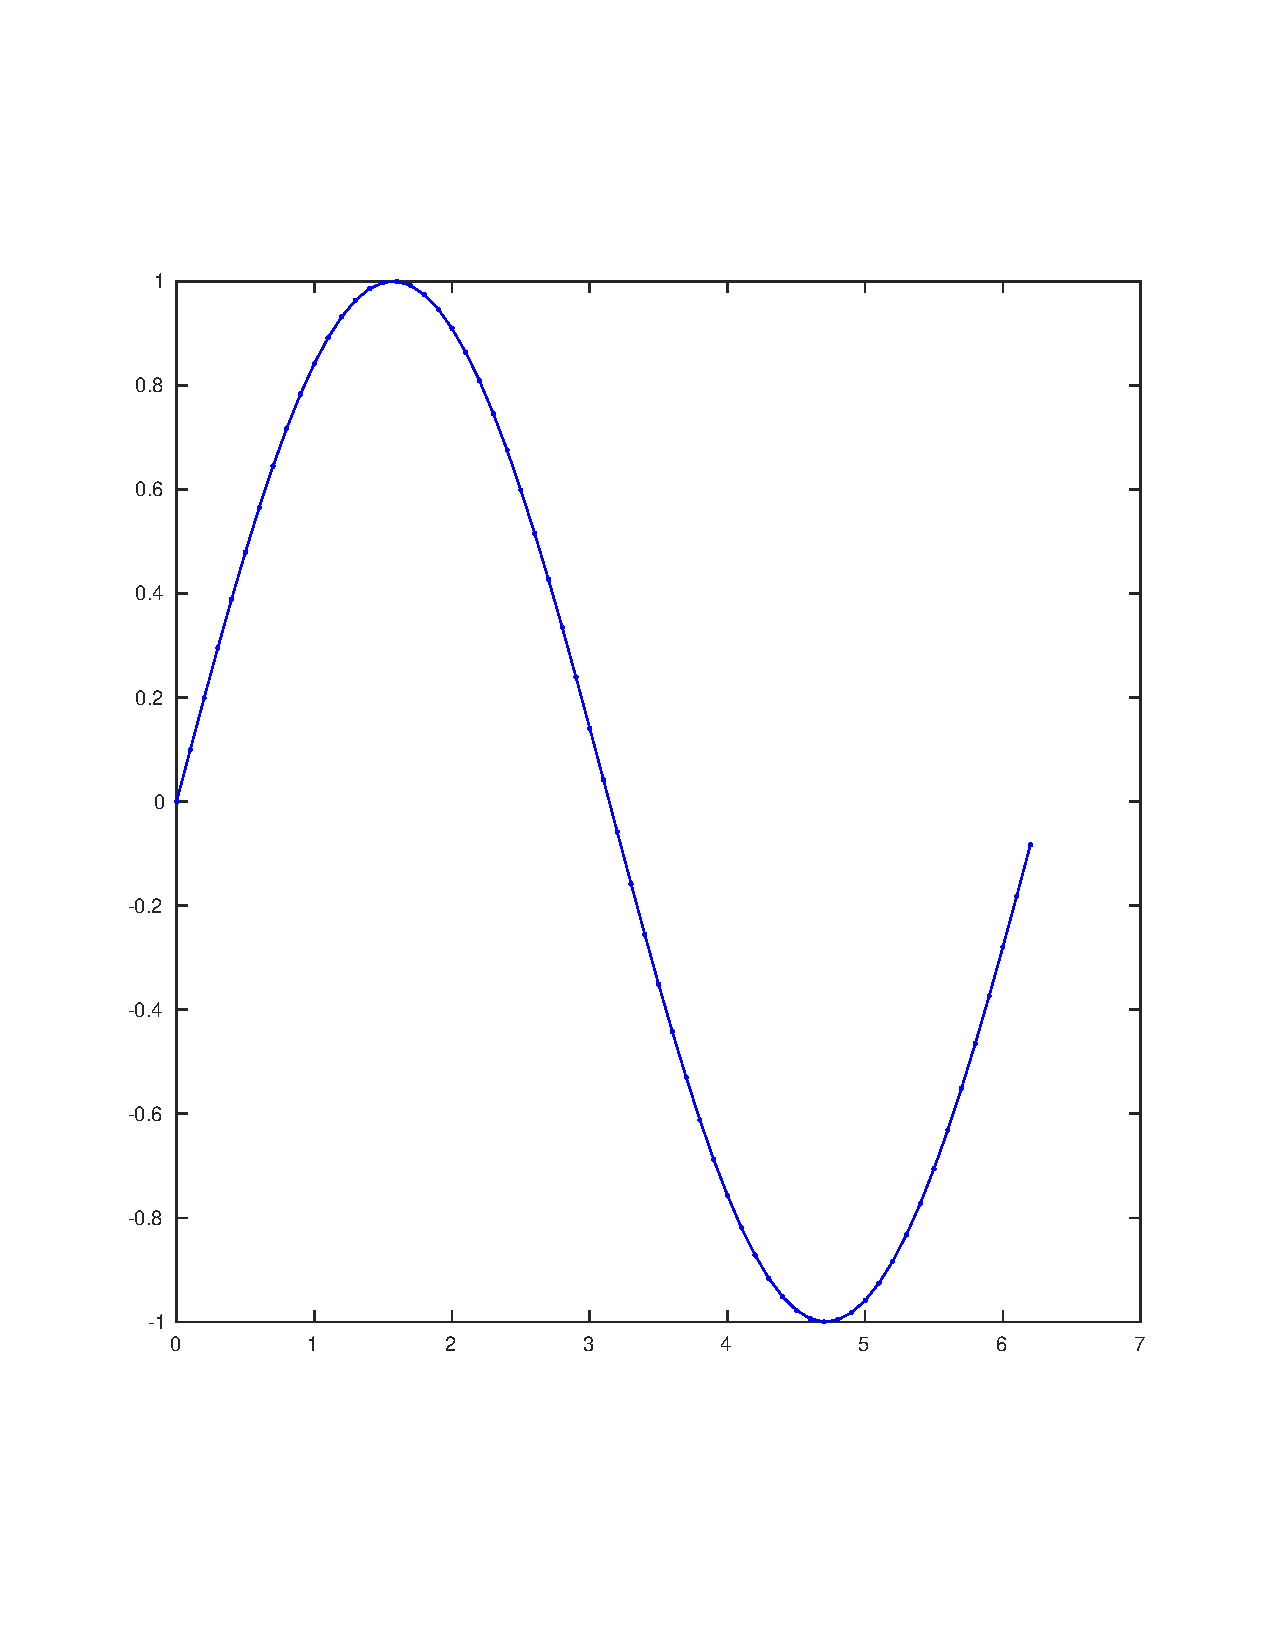
\includegraphics
	[width=0.3\textwidth,
	clip=true,
	trim=2cm 5cm 2cm 1cm]{sine.pdf}
\end{center}   
	\caption{$f(x) = \sin(x)$}.
\end{figure}
Some text after the figure.

Some text before figure with [H] specifier.
\begin{figure}[H]
\begin{center}
	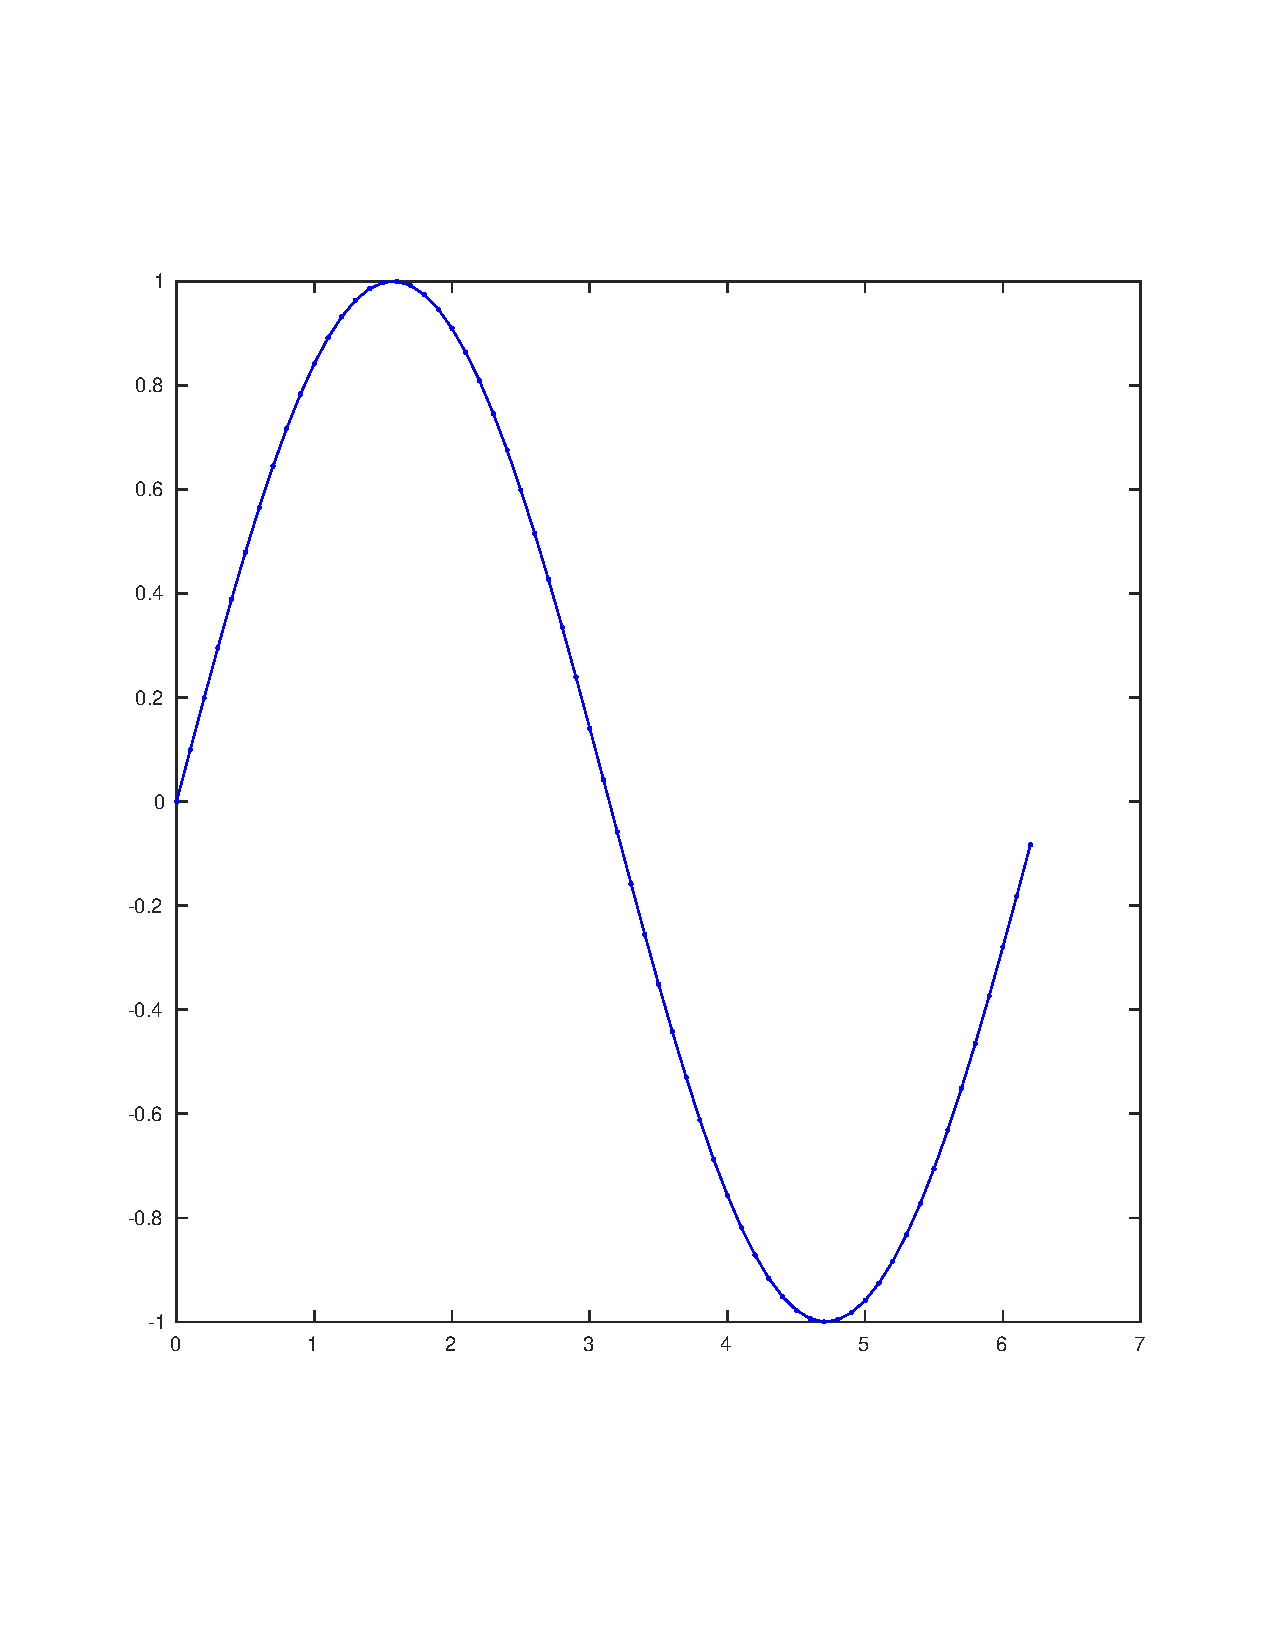
\includegraphics
	[width=0.3\textwidth,
	clip=true,
	trim=2cm 5cm 2cm 1cm]{sine.pdf}
\end{center}   
	\caption{$f(x) = \sin(x)$}.
\end{figure}
Some text after figure with [H] specifier.

\end{document}